\chapter{Szövegosztályozási feladat és módszerek}

Ebben a fejezetben a kontextus megteremtése érdekében a természetes nyelvfeldolgozás és a szövegosztályozás alapfogalmai kerülnek bevezetésre. Ezt követően a szövegosztályozás folyamatáról esik szó. Végül a felhasznált módszerek részletezése következik.

\section{Természetes nyelvfeldolgozás}

A természetes nyelvfeldolgozás olyan tudományág, amely lehetővé teszi a számítógépek és digitális rendszerek számára az emberi nyelv értelmezését, megértését és generálását. Integrálja a számítógépes nyelvészetet, a szabályalapú megközelítéseket, a statisztikai modellezést, valamint a korszerű mélytanulási technikákat~\cite{ibmThinkNLP}.

A természetes nyelvfeldolgozás területén folyó kutatások döntő szerepet játszottak a generatív mesterséges intelligencia kifejlődésében, elősegítve a nagy nyelvi modellek kifinomult kommunikációs képességeit, amelyek képesek szöveges és beszélt nyelv értelmezésére, generálására és összetett feladatok végrehajtására~\cite{ibmThinkNLP}.

\section{Szövegosztályozás}

A szövegosztályozás egy olyan folyamat, amely során egy dokumentumot automatikusan egy vagy több kategóriába sorolnak. Létezik felügyelt és nem felügyelt változata.

A \textbf{felügyelt gépi tanulás} (Supervised Learning) módszer alapja a dokumentum belső jellemzőinek elemzése, majd egy előre címkézett adathalmaz segítségével modell létrehozása a dokumentum és a kategória közötti kapcsolatok feltérképezésére~\cite{wang2023textclassificationnlp}.

Vannak technikák, amelyek nem igénylik a címkézett adathalmazon tanított modellek használatát, azonban a dolgozat nem tér ki ezek részletezésére.

A szövegosztályozás jelentősége az \textbf{adatrobbanás korszakával} (Era of Big Data) tovább nőtt, hiszen lehetővé teszi a strukturálatlan szöveges adatok hatékony szervezését és feldolgozását. Számos tanulmány rámutat arra, hogy a szövegosztályozás nem csupán egy a sok természetes nyelvfeldolgozás feladat közül, hanem a terület alapvető építőeleme. \cite{li2022surveytextclassification} megállapítja, hogy „a szövegbesorolás a természetes nyelvfeldolgozás legfontosabb és legalapvetőbb feladata” (saját fordítás).

\section{A szövegosztályozás folyamata}

A folyamat tipikusan több egymást követő lépésből áll, melyet \mref{fig:text-classification-flow} szemléltet. Kezdve a \textbf{szöveg előfeldolgozásával} (preprocessing), amely magában foglalja a tokenizálást, a stop-szavak eltávolítását, a szöveg kisbetűsítését, valamint a szótövezést vagy a lemmatizálást. Az előfeldolgozás célja egy egységes, zajtól megtisztított és könnyen feldolgozható szövegállomány előállítása, amely stabil alapot biztosít a további lépésekhez. Ezt követi a \textbf{jellemzőkinyerés} (feature extraction), amelynek során a dokumentumok numerikus reprezentációra alakíthatók. Ez a reprezentáció teszi lehetővé, hogy a különböző gépi tanulási algoritmusok a szöveg struktúráját és tartalmi jellemzőit kvantitatív módon értelmezzék.

\begin{figure}[htbp]
  \centering
  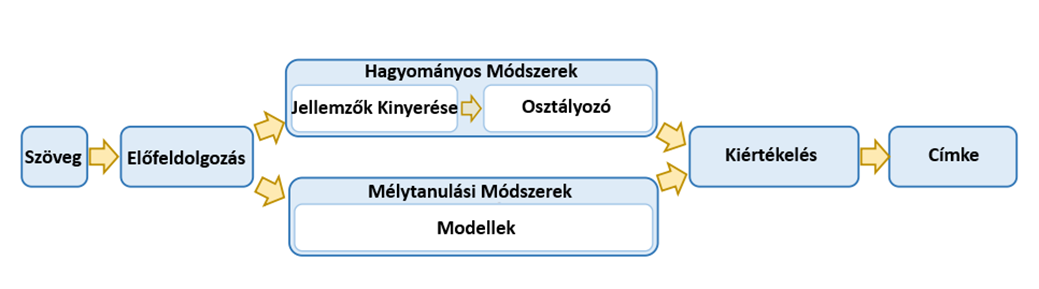
\includegraphics[width=\linewidth]{images/text_classification_flowchart}
  \caption{A szövegosztályozás tipikus folyamata: \emph{szöveg} és \emph{előfeldolgozás}, majd a \emph{hagyományos módszerek} (jellemzőkinyerés, osztályozó) és a \emph{mélytanulási módszerek} (modellek) párhuzamos ága, ezután \emph{kiértékelés} és \emph{címke} kimenet. \emph{Forrás:}~\cite{li2022surveytextclassification}.}
  \label{fig:text-classification-flow}
\end{figure}

Az osztályozási modell létrehozása előtt általában sor kerül a tanított modell \textbf{kiértékelésére} (evaluation), amely során különböző teljesítménymutatók -- például pontosság, visszahívás, F1-mérték vagy \textbf{görbe alatti terület} (Area Under the Curve, AUC) -- segítségével vizsgálható, hogy a modell milyen mértékben képes a különböző kategóriák helyes elkülönítésére. A kiértékelés elengedhetetlen lépés annak meghatározásához, hogy a modell alkalmas-e éles környezetben történő alkalmazásra, illetve hogy szükség van-e további finomhangolásra vagy alternatív jellemzők használatára.

A folyamat végén az \textbf{osztályozó} (classifier) a dokumentumot a megfelelő \textbf{címkéhez} (label) rendeli, amely a későbbi elemzési feladatok kiindulópontja lehet. A szövegosztályozás eredményei többféle további feldolgozást támogatnak, például \textbf{érzelmi állapotok feltárását} (sentiment analysis), \textbf{témaazonosítást} (topic analysis), spam- vagy anomáliaészlelést, valamint nagy szövegkorpuszok strukturálását és információvisszakeresési rendszerek hatékonyságának javítását. A címkézett adatok ezen túlmenően alapot biztosítanak prediktív modellekhez, ajánlórendszerekhez, illetve bármely olyan automatizált folyamat számára, ahol nagy mennyiségű szöveges adat gyors és megbízható kategorizálása szükséges.

\section{Áttérés a hagyományos módszerekről a mélytanulási módszerekre}

\cite{li2022surveytextclassification} szerint „az 1960-as évektől a 2010-es évekig a hagyományos szövegbesorolási módszerek domináltak” (saját fordítás), és a mélytanulási módszerekre való áttérés 2010-ben kezdődött. A hagyományos módszerek statisztikán alapulnak, és a korábbi szabályalapú módszerekhez képest nagyobb pontosságot és stabilitást mutattak. Az adatrobbanás korában azonban a manuális jellemzőkinyerés költséges és időigényes, a statisztikai megközelítések pedig figyelmen kívül hagyják a szöveges adatok természetes szekvenciális szerkezetét vagy kontextusbeli információit.

A hagyományos megközelítésekkel szemben a mélytanulási módszerek kiküszöbölik a kézzel készített szabályok és kézi jellemzőkinyerés szükségességét, mivel képesek az adatokból automatikusan, szemantikailag gazdag és kontextusérzékeny reprezentációkat tanulni. Ez a tulajdonság lehetővé teszi a \textbf{mély neurális hálózatok} (Deep Neural Network, DNN) számára, hogy olyan összetett nyelvi mintázatokat, hosszú távú függőségeket és finom szemantikai különbségeket is megragadjanak, amelyeket a hagyományos technikák jellemzően nem képesek megfelelő pontossággal modellezni. Ennek következtében a szövegosztályozás területén végzett jelenkori kutatások döntő része mély neurális hálózatokra épül, amelyek adatvezérelt architektúrákként automatikusan képesek hierarchikus jellemzők kinyerésére, és számos alkalmazási területen a legkorszerűbb teljesítményt biztosítják. Ugyanakkor a mélytanulási modellek hatékony működéséhez általában jelentős számítási kapacitásra és nagy méretű, annotált tanítóadatokra van szükség. Emiatt a \textbf{hagyományos gépi tanulási} (Traditional Machine Learning) módszerek iránti érdeklődés elsősorban azokban a szcenáriókban maradt fenn, ahol a számítási erőforrások korlátozottak, az adatmennyiség csekély, vagy valós idejű feldolgozási követelmények teszik szükségessé a könnyebb, kompaktabb modellek alkalmazását.

Két nagy osztályba sorolhatók a szövegosztályozási technikák, az \textbf{adattudomány} (Data Science) és a \textbf{mesterséges intelligencia} (Artificial Intelligence) alá~\cite{taha2024textclassificationsurvey}.

Itt érdemes megemlíteni, hogy ez a két osztály nem diszjunkt, hanem az adattudomány egy szélesebb terület, amelynek egyik eszköze lehet a mesterséges intelligencia. Ezt a következtetést definíciójukból le lehet vonni.

Az adattudomány „Olyan tudományág, amely tudományos módszereket, folyamatokat és rendszereket alkalmaz az adatokból származó ismeretek és betekintések kinyerésére”~\cite{uscensusDatascience} (saját fordítás).

A mesterséges intelligencia egyik definíciója: „Egy technológia, amely felruházza a számítógépeket és gépeket az emberi tanulás, megértés, problémamegoldás, döntéshozatal, kreativitás és önállóság utánzásának képességével”~\cite{ibmThinkAI} (saját fordítás).

\begin{figure}[htbp]
  \centering
  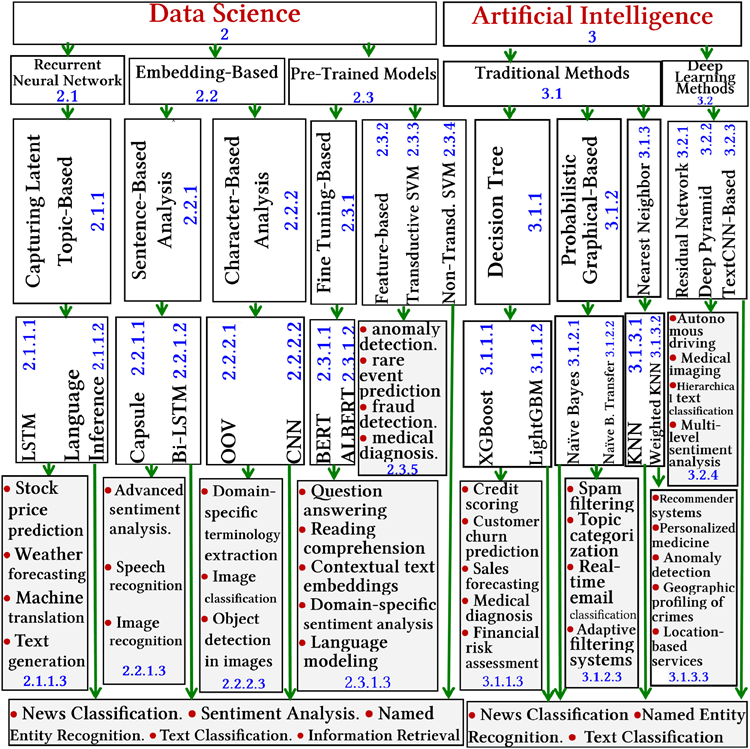
\includegraphics[width=\linewidth]{images/text_classification_taxonomy}
  \caption{A szövegosztályozási módszerek taxonómiája. \emph{Forrás:}~\cite{taha2024textclassificationsurvey}.}
  \label{fig:text-classification-taxonomy}
\end{figure}
